\documentclass{article}
\usepackage[margin=1in]{geometry}
\usepackage{amsmath}
\usepackage{graphicx}
\usepackage{listings}
\usepackage{xcolor}
\usepackage{hyperref}
\definecolor{mygreen}{rgb}{0,0.6,0}
\definecolor{mygray}{rgb}{0.5,0.5,0.5}
\definecolor{mymauve}{rgb}{0.58,0,0.82}

\lstset{ %
  backgroundcolor=\color{white},   % choose the background color; you must add \usepackage{color} or \usepackage{xcolor}
  basicstyle=\scriptsize\ttfamily,    % the size of the fonts that are used for the code
  breakatwhitespace=false,         % sets if automatic breaks should only happen at whitespace
  breaklines=true,                 % sets automatic line breaking
  captionpos=b,                    % sets the caption-position to bottom
  commentstyle=\color{mygreen},    % comment style
  deletekeywords={},            % if you want to delete keywords from the given language
  escapeinside={\%*}{*)},          % if you want to add LaTeX within your code
  extendedchars=true,              % lets you use non-ASCII characters; for 8-bits encodings only, does not work with UTF-8
  frame=shadowbox,                    % adds a frame around the code
%  framexleftmarign=5mm,
  xleftmargin=10pt,
  xrightmargin=10pt,
  rulesepcolor=\color{gray},
  keywordstyle=\color{blue},       % keyword style
  language=Octave,                 % the language of the code
  morekeywords={*,...,fit,predint,export\_fig},            % if you want to add more keywords to the set
%  numbers=left,                    % where to put the line-numbers; possible values are (none, left, right)
  numbers=none,
  numbersep=5pt,                   % how far the line-numbers are from the code
  numberstyle=\tiny\color{mygray}, % the style that is used for the line-numbers
  rulecolor=\color{black},         % if not set, the frame-color may be changed on line-breaks within not-black text (e.g. comments (green here))
  showspaces=false,                % show spaces everywhere adding particular underscores; it overrides 'showstringspaces'
  showstringspaces=false,          % underline spaces within strings only
  showtabs=false,                  % show tabs within strings adding particular underscores
  stepnumber=1,                    % the step between two line-numbers. If it's 1, each line will be numbered
  stringstyle=\color{mymauve},     % string literal style
  tabsize=4,                       % sets default tabsize to 4 spaces
  caption=\lstname                   % show the filename of files included with \lstinputlisting; also try caption instead of title
}


\title{1.723 HW2}
\author{Sachith  Dunatunga}

\begin{document}
\maketitle

%
%
%
\section{Problem 1}
From class, we know the general form of the dispersion tensor in indicial notation is given by
\begin{align}
    \mathbf{D}_{ij} = \alpha_T \sqrt{u_i u_j} \delta_{ij} + (\alpha_L - \alpha_T) \frac{u_i u_j}{\sqrt{u_k u_k}}.
\end{align}

Since $|\mathbf{u}| = \sqrt{u_k u_k} = \sqrt{u_x^2 + u_y^2}$ in 2D, we can write
\begin{align}
    \begin{bmatrix}
        D_{xx} & D_{xy} \\
        D_{yx} & D_{yy}
    \end{bmatrix} &= \frac{1}{\sqrt{u_x^2 + u_y^2}}
    \begin{bmatrix}
        u_x^2 \alpha_L  + u_y^2 \alpha_T & u_x u_y (\alpha_L - \alpha_T) \\
        u_x u_y (\alpha_L - \alpha_T) & u_x^2 \alpha_T + u_y^2 \alpha_L
    \end{bmatrix}
\end{align}
\section{Problem 2}
\subsection{Part 1}
We first used datathief to get the coordinates of the points shown in figure \ref{fig:datathief}.
\begin{figure}[!h]
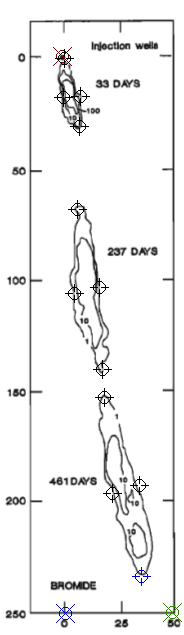
\includegraphics[scale=1.0]{dt.png}
\centering
\label{fig:datathief}
\end{figure}

Centroids of these three groups of points are calculated, and a line of best fit going through the origin is calculated for both the x and y directions.
The coefficients of these fits are the interstitial velocity $\mathbf{v} = (0.0581, 0.42534)\ [\mathrm{m} / \mathrm{day}]$.
The darcy velocity is related to the interstitial velocity through the porosity via $\mathbf{v} \phi = \mathbf{u} = (0.0227, 0.1659)\ [\mathrm{m} / \mathrm{day}]$.

\subsection{Part 2}
Using the same points as from before, we calculated the longitudinal distance and transverse distance of the plume at each time.
We then do another linear regression passing through the origin of the form  $y = Dt$, where $y = \frac{1}{2}l^2$, for both the longitudinal and transverse directions.
We then assume that the longitudinal direction is the direction of the darcy velocity (to simplify analysis), and take
\begin{align}
\alpha_L &= \frac{D_L}{|\mathbf{u}|} = 48.84\ [\mathrm{m]}\\
\alpha_T &= \frac{D_T}{|\mathbf{u}|} = 1.280\ [\mathrm{m}]
\end{align}
These values seem large, but dispersivity can vary massively so I do not know if they are unreasonable.
The large anisotropy, which is evident from the shape change, is captured by having a much smaller value of $\alpha_T$ than $\alpha_L$.
The spreadsheet with the intermediate calculations is attached.


% \appendix
% \section{Programs}
% \lstinputlisting[label=code:plotting]{sandstone_figures.py}

\end{document}
